\documentclass[tikz, border = 2pt]{standalone}

%---------------------------------------------------------------------------%
% PACKAGES                                                                  %
%---------------------------------------------------------------------------%

%----- MATH
%---------------------------------------------------------------------------%
\usepackage{amsmath, amssymb}

%----- FIGURES
%---------------------------------------------------------------------------%
\usepackage{pgfplots}
\pgfplotsset{compat=1.13}
\tikzset{declare function={	normcdf(\x,\m,\s)=1/(1 + exp(-0.07056*((\x-\m)/\s)^3 - 1.5976*(\x-\m)/\s));	}}

\begin{document}

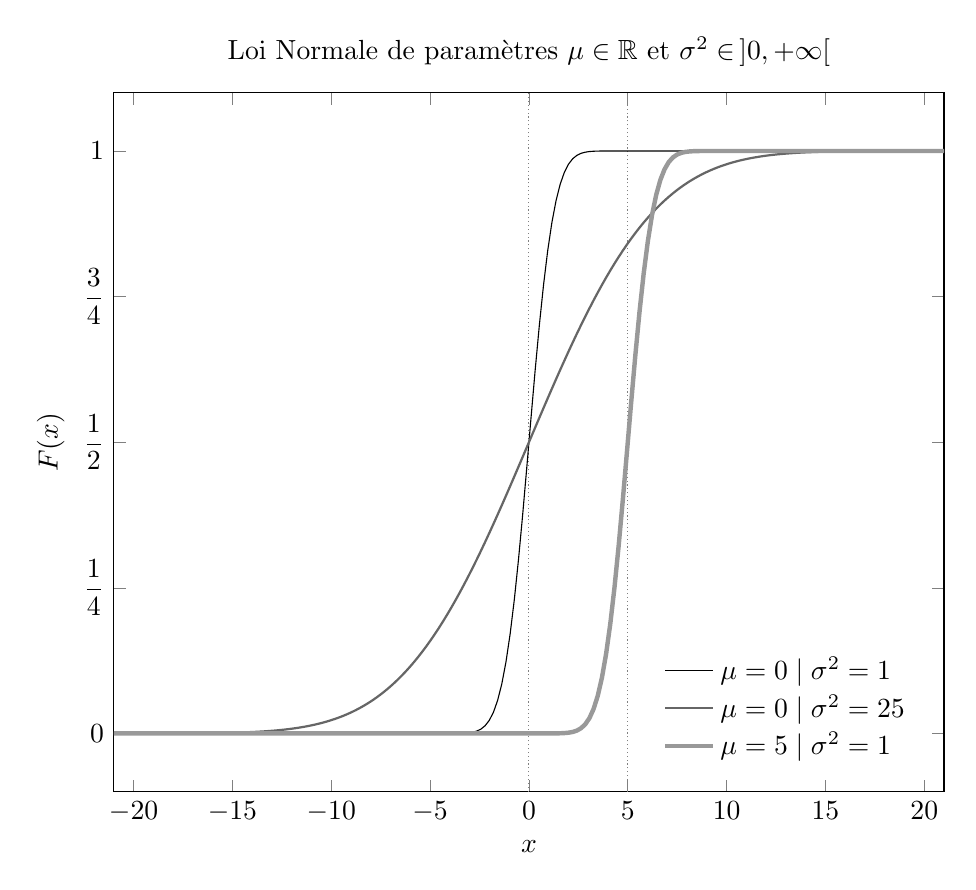
\begin{tikzpicture}
\begin{axis}[width = \textwidth,
title style = {align = center},
title={Loi Normale de param\`etres $\mu \in \mathbb{R}$ et $\sigma^2 \in\, ]0,+\infty[$},
xlabel={$x$},
ylabel={$F(x)$},
legend pos = south east,
legend style = {draw=none},
legend cell align = left,
xmin = -21,
xmax = 21,
ytick = {0,0.25,0.5,0.75,1},
yticklabels = {$0$, $\dfrac{1}{4}$, $\dfrac{1}{2}$, $\dfrac{3}{4}$, $1$},
ylabel near ticks,
domain = -21:21
]
\draw[black!50, densely dotted] (0,-.1) -- (0,1.1);
\draw[black!50, densely dotted] (5,-.1) -- (5,1.1);
\addplot[black, samples = 200] {normcdf(x,0,1)};
%
\addplot[black!60, thick, samples = 200] {normcdf(x,0,5)};
%
\addplot[black!40, ultra thick, samples = 200] {normcdf(x,5,1)};
%
\legend{{$\mu=0 \mid \sigma^2 = 1$}, {$\mu=0 \mid \sigma^2 = 25$}, {$\mu=5 \mid \sigma^2 = 1$}}
\end{axis}
\end{tikzpicture}

\end{document}